\section{Estrellas de neutrones}\label{sc:intro}

Las estrellas de neutrones aparecen en el universo como el remanente de la muerte de una estrella masiva (pero no tan masiva como para convertirse en un agujero negro).
Cuando nace una estrella consume principalmente Hidrógeno, produciendo Helio en el proceso.
Unos $10^{10}$ años después el Hidrógeno se agota y la estrella, que ya no puede compensar la compresión gravitatoria, se contrae y se calienta.
Esto le permite comenzar a fusionar Helio, que vuelve a generar suficiente presión para evitar el colapso gravitatorio.
A medida que envejece, una estrella va consumiendo y agotando sucesivamente hidrógeno, helio, carbono, neón, oxígeno y silicio.
Cada vez que la estrella agota un tipo de combustible se produce el proceso mencionado: el núcleo se contrae, se calienta y comienza a consumir un nuevo combustible que, generalmente, es el producto de la fusión del anterior.
Esto se conoce como la ``secuencia principal'' de una estrella~\cite{woosley_physics_2005}.
Para poder fusionar elementos cada vez más pesados, una estrella requiere mayor temperatura, y sólo estrellas muy masivas (con masa mayor a 8 veces la masa solar) peuden completar la secuencia.
El producto de la fusión de silicio (la última etapa de la secuencia) es principalmente hierro y, dada su alta energíá de unión, no es posible extraerle energíá por fusión.
En la etapa del silicio (que dura apenas un par de semanas), casi toda la presión que evita el colapso es provista por un gas degenerado de electrones.
Eventualmente el núcleo, formado principalmente por hierro, alcanza una masa de $1.5\,M_\odot$, con un tamaño similar al de la tierra y una densidad superior a $10^{10}\,\text{g/cm}^{3}$.

A esas densidades, los electrones comienzan a ser capturados por los núcleos de hierro, aumentando la proporción de neutrones y privando al núcleo estelar de la presión ejercida por el gas de electrones.
Esto precipita el colapso gravitatorio del núcleo, que comienza a comprimirse violentamente a una velocidad de $0.25c$.
Eventualmente la componente repulsiva de la interacción nuclear detiene la compresión y el núcleo comienza a expandirse.
Todo este proceso lleva del orden de un segundo.
Durante esta etapa, el núcleo emite una gran cantidad de neutrinos, presuntamente originados en el proceso de Urca:
\begin{equation}
  p + e\rightarrow n + \nu_e
\end{equation}
Por mecanismos que no están del todo claros, la expansión se detiene, conformando una proto-estrella de neutrones caliente (con temperaturas de entre $20$ y $50\,\text{MeV}$).
Esa proto-estrella de neutrones va acreciendo material de las capas exteriores de la estrella y, si no se convierte en un agujero negro, se enfría hasta estabilizarse (principalmente a través de la emisión de neutrinos) formando un núcleo rico en neutrones de aproximadamente $10\,\text{km}$ de radio: una estrella de neutrones propiamente dicha.
Durante esta etapa, la proto-estrella de neutrones emite hasta un 10\% de su masa en reposo en forma de neutrinos, y se cree que la interacción de estos neutrinos con el material de las capas exteriores de la estrella produce la Super Nova, a pesar de que no hay consenso sobre los detalles del mecanismo~\cite{woosley_physics_2005, bethe_supernova_1990}.
También está en discusión el proceso de Urca como mecanismo de enfriamiento~\cite{piekarewicz_proton_2012, lattimer_direct_1991}, puesto que para algunos modelos de ecuación de estado la fracción de protones en equilibrio no sería suficiente como para producir la cantidad de neutrinos necesaria.
Durante este colapso, una gran parte de los electrones y los protones se transforman en neutrones a través de la captura de electrones, emitiendo neutrinos.
Debido a esto, la masa residual tiende a tener un exceso de neutrones por sobre protones, de ahí el nombre estrellas de neutrones.
Estas estrellas de neutrones entonces contienen tanto protones como neutrones, pero además son eléctricamente neutros debido a los electrones: la carga neta es cero.

La masa de una estrella de neutrones es de entre 1 y 3 masas solares y su radio de cerca de $10\,\text{km}$, lo que resulta en una densidad de $\rho \simeq 10^{15}\,\text{g/cm}^3$, aproximdadmente 20 veces mayor que la de los nucleos usuales.
%Consideraciones energéticas indican que los núcleos de las estrellas de neutrones están cubiertos por una \emph{corteza} de aproximadamente $1\,\text{km}$ de espesor, donde los neutrones producidos por decaimiento $\beta$ forman materia nuclear rica en neutrones.
Su estructura puede dividirse en dos partes, de acuerdo a modelos actuales~\cite{page_minimal_2004, geppert_temperature_2004}: la \emph{corteza}, de aproximadamente $1.5\,\text{km}$ de espesor y con una densidad de hasta la mitad de la densidad normal nuclear $\rho_0$; y el \emph{núcleo}, donde la estructura es aún desconocida y se mantiene altamente especulativa~\cite{akmal_equation_1998, ravenhall_structure_1983, oyamatsu_nuclear_1993, woosley_physics_2005}.

La densidad de dicha corteza toma los valores de la densidad nuclear normal ($\rho \simeq 10^{14}\,\text{g/cm}^3$ o $ \rho \simeq \rho_0=0.15 \text{fm}^{-3}$) a una profundidad $d \simeq 1\,\text{km}$, la densidad de \emph{neutron drip} ($\rho\simeq 4 \cdot 10^{11}\,\text{g/cm}^3$) a $d\simeq 0.5\,\text{km}$, y una mezcla de nucleos ricos en neutrones con densidades decrecientes hasta ser prácticamente cero en lo que se conoce como el envoltorio de la estrella de neutrones.
Ravenhall \emph{et al.} en Ref.~\cite{ravenhall_structure_1983} y Hashimoto \emph{et al.} en Ref.~\cite{hashimoto_shape_1984} propusieron que la corteza de las estrellas de neutrones está compuesta por estructuras conocidas como \emph{pasta nuclear}.

Varios modelos han sido desarrollados para estudiar la pasta nuclear, y han mostrado que estas estructuras aparecen debido al juego entre las fuerzas nuclears y las de Coulomb en un medio infinito.
De cualquier modo, cómo dependen los observables de diferentes cantidades termodinámicas no ha sido estudiado en profundidad.
Los trabajos originales de Ravenhall \emph{et al.}~\cite{ravenhall_structure_1983} y Hashimoto \emph{et al.}~\cite{hashimoto_shape_1984} utilizaban un modelo de gota líquida compresible, y mostraron que las \emph{fases de pasta}
--\emph{lasagna}, \emph{spaghetti} y \emph{gnocchi}-- son soluciones al estado fundamental de la materia de estrellas de neutrones.
De ahí en adelante, se han tomado distintos enfoques que clasificaremos en dos categorías: campo medio o microscópico.

Los trabajos de campo medio incluyen el modelo de la gota líquida, de Lattimer \emph{et al.}~\cite{page_minimal_2004}, Thomas-Fermi, de Williams y Koonin~\cite{williams_sub-saturation_1985}, entre otros~\cite{oyamatsu_nuclear_1993, lorenz_neutron_1993, cheng_properties_1997, watanabe_thermodynamic_2000, watanabe_electron_2003, nakazato_gyroid_2009}.
Los modelos microscópicos incluyen Dinámica Molecular Cuántica (QMD por sus siglas en inglés), usado por Maruyama \emph{et al.}~\cite{maruyama_quantum_1998, kido_md_2000} y por Watanabe~\emph{et al.}\cite{watanabe_structure_2003}, el Potencial Simple Semiclásico (SSP), utilizado por~\emph{et al.}~\cite{horowitz_nonuniform_2004} y Dinámica Molecular Clásica (CMD), utilizado en nuestros trabajos previos~\cite{dorso_topological_2012}.
De todos los modelos utilizados para estudiar las estrellas de neutrones, las ventajas de los modelos clásicos o semiclásicos son la accesibilidad a las posiciones y velocidades de todas las partículas y el hecho de que no se debe especificar \emph{a priori} ninguna forma específica, a diferencia de la mayoría de los modelos de campo medio.
Esto permit eestudiar la estructura de la ma de estrellas de neutrones desde un punto de vista de las partículas.
En estos modelos, la repulsión de Pauli entre nucleones del mismo isospín es, o bien considerado en la interacción nuclear, o bien agregado como un término aparte~\cite{dorso_classical_1988}.

La multifragmentación en sistemas nucleares fue estudiada
antes~\cite{bonasera_critical_2000, chikazumi_quantum_2001}, pero, a
diferencia de las colisiones, fue en mayor medida con materia nuclear (sin la interacción de Coulomb).
En un reciente trabajo de Caplan et al~\cite{caplan_pasta_2015}, se estudió la materia de estrellas de neutrones expandiéndose como posible explicación para la nucleosíntesis en colisiones de estrellas de neutrones y en otro trabajo, de este grupo~\cite{alcain_dynamics_2017}, la formación de los fragmentos en la expansión.

La compresión de la materia de estrellas de neutrones durante la colisión de dos estrellas es una posible fuente para nucleos a través del \emph{r-process}, como fue discutido inicialmente en Ref.~\cite{lattimer_black-hole-neutron-star_1974}.
De acuerdo a modelos hidrodinámicos~\cite{goriely_r-process_2011}, éstos tienen coeficientes de expansión típicos de  $\eta = 10^{-21}\,\text{c/fm} < \eta < 4\cdot 10^{-20}\,\text{c/fm}$.
Inspirados por la colisión de estrellas de neutrones, desarrollamos un estudio en la fragmentación de materia de estrellas de neutrones en expansión.

\section{Dinámica de los nucleones}\label{sc:nucleon}
Para estudiar la estructura nuclear de la corteza de las estrellas de neutrones es necesario comprender el comportamiento de los nucleones (es decir, protones y neutrones) a las densidades y temperaturas típicas de las capas externas de las estrellas.
Este conocimiento viene de décadas de estudio de la dinámica de nucleones a través del uso de modelos computacionales que han evolucionado, siendo cada vez más complejos.
En esta sección, revisamos esta evolución de los modelos, presentando una sinopsis de los modelos existentes y terminando con el modelo utilizado a lo largo de este trabajo: Dinámica Molecular Clásica (CMD).

\subsection{Evolución de los modelos}
Varios enfoques se han utilizado para simular el comportamiento de la materia nuclear, especialmente en reacciones.
Los estudios iniciales, en mayor parte estadísticos, se desarrollaron hacia la década de 1980.
Éstos carecían de interacciones entre fragmentos y la dinámica de fragmentos luego de la colisión.
En la década del 1990 se agregaron estos efectos, resultando así en modelos más robustos~\cite{barz_cluster_1996}.
Todos estos modelos, sin embargo, estaban basados en geometrías idealizadas e ignoraban importantes fluctuaciones de forma y los efectos de la cinemática en la reacción.
Desde el lado de la teoría de transporte, se desarrollaron modelos hacia el fin de la década de 1990 que se basaron en modelos cuánticos, clásicos y semiclásicos.
Debido a su uso actual en materia de estrellas de neutrones, es importante realizar una comparación entre estos modelos.

Comenzando con el semiclásico, una clase de modelos conocidos genéricamente como BUU está basado en la ecuación cinética de Vlasov-Nordheim~\cite{nordheim_kinetic_1928}, también conocida como Boltzmann-Uehling-Uhlenbeck~\cite{uehling_transport_1933}.
Estos modelos siguen numéricamente la evolución de la función de Wigner $f(\mathbf{r},\mathbf{p})$ (densidad de un cuerpo en el espacio de fases), bajo un potencial medio $U(\mathbf{r})$ para obtener una descripción de la probabilidad de encontrar una partícula en un punto del espacio de fases.
La interpretación semiclásica constituye la ventaja principal del modelo BUU, aunque la limitación de utilizar sólo un campo medio implica que los fragmentos no se desarrollan espontáneamente.
Para poder producir fragmentos, deben ser agregadas fluctuaciones \emph{ad hoc}, y aún más términos deben ser agregados para obtener características más realistas.

En el lado cuántico (que, en realidad, son modelos efectivamente semiclásicos), los modelos de dinámica molecular, llamados QMD genéricamente, resuelven las ecuaciones de movimiento de ``paquetes de onda'' de nucleones moviéndose dentro de campos medios (derivados de la funcial de energía de Skyrme).
Este método permite la imposición de un mecanismo de bloqueo del estilo de Pauli, secciones eficaces dependientes del isospin, dependencia de la interacción con el momento relativo de las partículas, entre otras.
La mayor ventaja de este modelo es que QMD es capaz de producir fragmentos, pero realiza una descripción pobre de las propiedades de los clusters y necesita métodos externos para quitarle el exceso de energía a los fragmentos que se forman~\cite{polanski_development_2005};
normalmente los fragmentos se construyen externamente a través de un modelo basado en distancias y momentos relativos.

También es de particular importancia para este trabajo el modelo de dinámica molecular clásico CMD, desarrollado por el grupo de Urbana~\cite{lenk_accuracy_1990} y diseñado para reproducir las predicciones de la ecuación de Vlasov-Nordheim y proveer una descripción más completa de las reacciones de iones pesados.
Este modelo se basa en el potencial de Pandharipande, que provee la interacción nuclear a través de una combinación de potenciales de tipo Yukawa seleccionados para que la materia nuclear infinita tenga valores adecuados para la densidad de equilibrio, energía por partícula y compresibilidad.

Problemas comunes tanto a BUU como a QMD son el fracaso en producir el número adecuado de fragmentoo, así como el uso de parámetros externos ajustables (como el tamaño de los paquetes de onda, el número de partículas de prueba, modificaciones sobre el capmo medio, masas efectivas y secciones eficaces).
Estos problemas no están presentes en CMD, que sin ningún tipo de parámetro extra, es capaz de describir la dinámica de la reacción en el espacio desde el comienzo hasta el final con valores adecuadios para la energía, la distribución espacial y en el espacio de momentos.
Intrínsicamente incluye todas las correlaciones de partículas a todos los niveles: dos cuerpos, tres cuerpos\ldots y puede describir sistemas nuclears que van desde nucleos fríos hasta decaimientos secundarios, parasadndo por transiciones de fase, flujo hidrodinámico y materia nuclear densa.

La única desventaja aparente del CMD es la falta de efectos cuánticos, como el bloqueo de Pauli, que a energías de excitación bajas no permite que se describa la estructura nuclear correctamente.
Afortunadamente, en colisiones, la gran deposición de energía implica una apertura del espacio de fases disponible y así se reduce el efecto de exclusión de Pauli~\cite{lopez_lectures_2000}, mientras que en entornos estelares, las colisiones que transfieren momentos dejan de ser un factor importante al decidir la configuración estable de la materia nuclear.
Independientemente de eso, el rol de los efectos cuánticos en colisiones de dos cuerpos, está incluído de forma efectiva ya que el potencial reproduce adecuadamente las secciones eficaces.
Más aún, un camino alternativo sería utilizar potenciales dependientes del momento (como el introducido por Dorso y Randrup~\cite{dorso_classical_1988}) cuando sea necesario.

A pesar de que ninguna teoría puede arrogarse una descripción perfecta de la materia nuclear, todos los enfoques tienen sus pros y contras y aparentar ser complementarios entre sí.

\subsection{Classical Molecular Dynamics}\label{ssc:cmd}
A lo largo de este trabajo utilizamos para modelar la dinámica de los nucleones el CMD.\@
Ha sido usado en varias reacciones de iones pesados para estudiar datos experimentales~\cite{chernomoretz_quasiclassical_2002}; identificar señales de transiciones de fase y otros fenómenos críticos~\cite{lopez_lectures_2000, barranon_searching_2001, dorso_selection_2001, barranon_critical_2003, barranon_time_2007}; y explorar la curva calórica~\cite{barranon_entropy_2004} y el \emph{isoscaling}~\cite{dorso_dynamical_2006, dorso_isoscaling_2011}.
CMD usa dos potenciales de dos cuerpos para describir la interacción entre nucleones, que son una combinación de potenciales de Yukawa:
\begin{align*}
  V^{\text{CMD}}_{np}(r) &=v_{r}\exp(-\mu_{r}r)/{r}-v_{a}\exp(-\mu_{a}r)/{r}\\
  V^{\text{CMD}}_{nn}(r) &=v_{0}\exp(-\mu_{0}r)/{r}
\end{align*}
donde $V_{np}$ es el potencial entre un neutron y un protón, mientras que $V_{nn}$ es la interacción repulisva tanto entre neutrones como entre protones.
El radio de corte es $r_c=5.4\,\text{fm}$, y para $r>r_c$ ambos potenciales se anulan.
Los parámetros de Yukawa $\mu_r$, $\mu_a$ y $\mu_0$ fueron determinados para resultar en una densidad de equilibrio de $\rho_0=0.16\,\text{fm}^{-3}$, una energía de ligadora $E(\rho_0)=16\,\text{MeV/nucleon}$ y una compresibilidad $\kappa=250\,\text{MeV}$.

Para simular un medio infinito, utilizamos este potencial bajo condiciones periódicas de contorno en cajas cúbicas, con distintos valores de fracción de protones, densidades y temperaturas.
Para realizar las simulaciones, usamos LAMMPS~\cite{plimpton_fast_1995} con su paquete de GPU~\cite{brown_implementing_2012}.

\subsubsection{Núcleos}
A pesar de que el estado a $T=0$ de esta materia nuclear clásica a densidades normales es un sólido con estructura cúbica simple, los sistemas nuclears pueden ser obtenidos agregando energía cinética a los nucleones.
Construimos estos núcleos confinando los nucleones en un potencial esférico y luego enfriándolos lentamente desde una temperatura elevada hasta que llegan a un estado de equilibrio ligado.
Luego retiramos el potencial confinante y enfriamos el sistema.
La figura~\ref{fig:binding} muestra las energías de ligadura de los estados fundamentales de los núcleos obtenidos con la fórmula de la gota líquida y con CMD; ver~\cite{dorso_isoscaling_2011} para más detalles.

\begin{figure}[h]
  \centering
  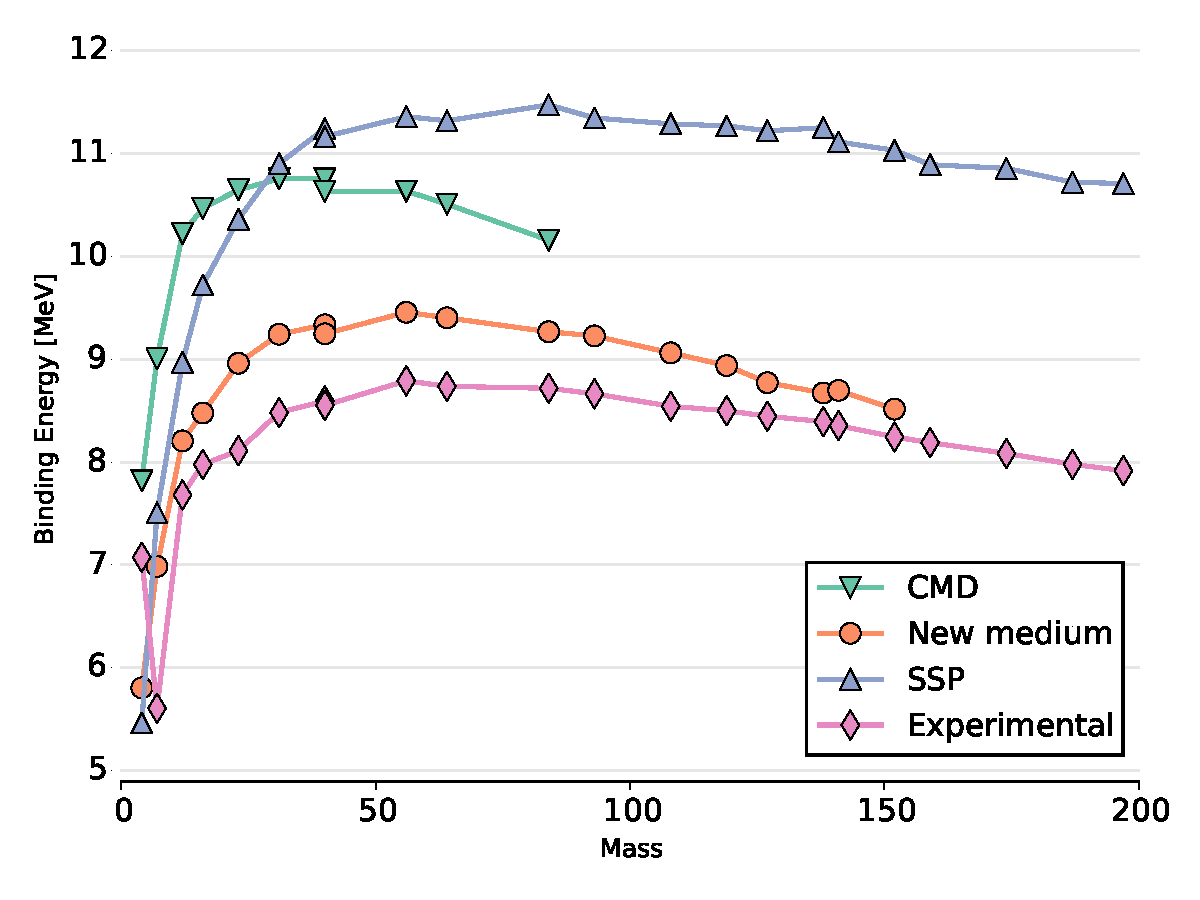
\includegraphics[width=0.8\columnwidth]{introduccion/binding}
  \caption{Energías de ligadura de núcelos obtenidas con CMD, extraída de Ref.~\cite{dorso_isoscaling_2011}.}
\label{fig:binding}
\end{figure}

\subsubsection{Colisiones}
Con respecto a las colisiones, estos potenciales reproducen las secciones eficaces de nucleon-nucleon para energías bajas e intermedias~\cite{lenk_accuracy_1990}, y fue utilizado extensivamente en el estudio de colisiones de iones pesados (ver Ref.~\cite{chernomoretz_quasiclassical_2002, barranon_time_2007}).
Para dichas reacciones, dos núcleos son impulsados uno contra el otro a una energía específica.
Entre colisión y colisión, el proyectil y el objetivo son rotados un con respecto al otro aleatoriamente.
La evolución del sistema se sigue utilizando un algoritmo de Verlet en velocidades, que es simpléctico y conserva la energía al 0.01\%.
A cualquier punto en el tiempo la posición y momento de los nucleones es conocida y puede ser transformada en información de fragmentos y partículas libres a través de distintas técnicas de reconocimiento de fragmentos~\cite{dorso_early_1993, dorso_when_1995, strachan_time_1997}.

Este método implica masas, momentos, energías de excitación y decaimientos secundarios comparables al experimental~\cite{belkacem_searching_1996,chernomoretz_quasiclassical_2002}.
La figura~\ref{fig:distribution}, por ejemplo, muestra las distribuciones de la velocidad paralela simuladas y experimentales obtenidas de la colisión de $\text{Ni+C}$ realizadas en el \emph{Coupled Tandem and Super-Conducting Cyclotron accelerators} de AECL en Chalk River~\cite{chernomoretz_quasiclassical_2002}.

\begin{figure}[h]
  \begin{subfigure}[h!]{\columnwidth}
    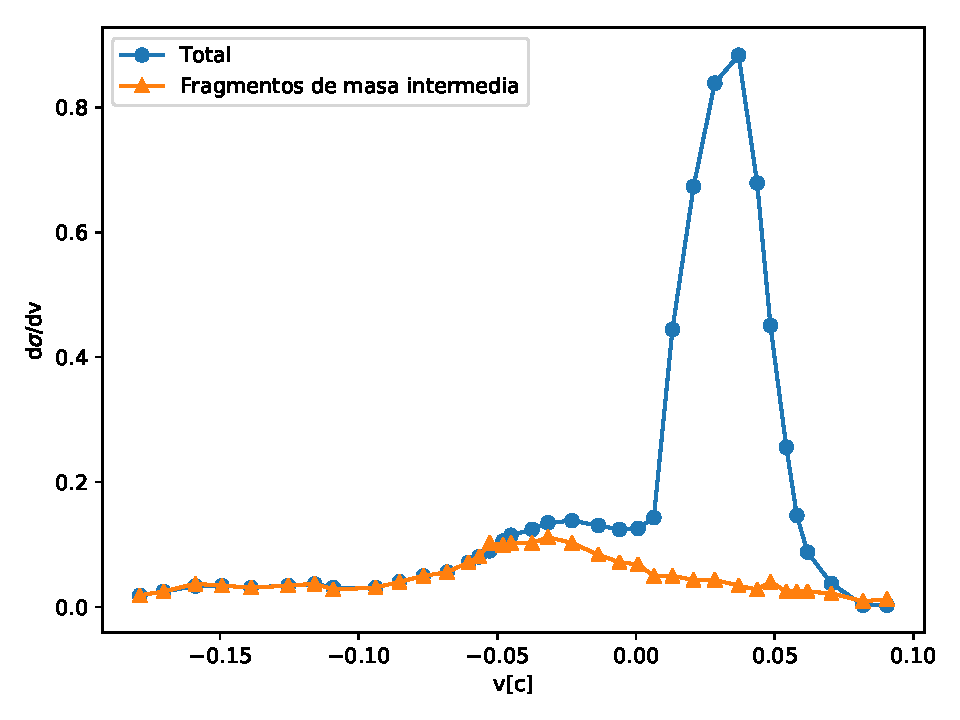
\includegraphics[width=\columnwidth]{introduccion/cherno_experiment}
    \caption{Resultados experimentales.}
    \label{sfig:exp}
  \end{subfigure}
  \begin{subfigure}[h!]{\columnwidth}
    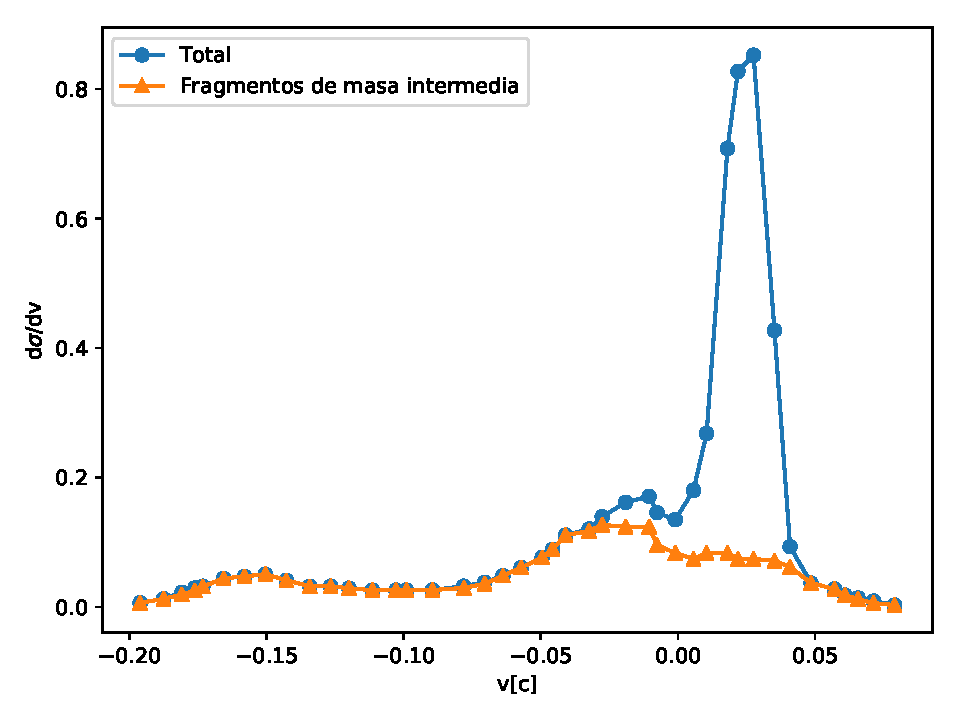
\includegraphics[width=\columnwidth]{introduccion/cherno_simulation}
    \caption{Resultados de la simulación.}
    \label{sfig:sim}
  \end{subfigure}
  \centering
  \caption{Distribuciones de velocidad paralela~\ref{sfig:exp} experimental y~\ref{sfig:sim} simulada para colisiones de ${}^{58}\text{Ni+C}$ collisions.}
  \label{fig:distribution}
\end{figure}


\subsubsection{Propiedades termostáticas de la materia nuclear}
Para estudiar las propiedades térmicas de la materia materia nuclear, calculamos la energía para distintos valores de temperatura.
Estos valores de energía por partícula $\epsilon(\rho,T)$ pueden ser utilizados para construir ajustes analítics, en el espíritu de los de Bertsch, Siemens y Kapusta~\cite{bertsch_nuclear_1983, kapusta_deuteron_1984,
  lopez_nuclear_1984}; estos ajustes, a su vez, pueden ser utilizados para encontrar otras variables termodinámicas, como por ejemplo la presión.

La figura~\ref{fig:energy_nm} muestra los resultados de este método aplicados por Giménez-Molinelli \emph{et al.}~\cite{gimenez_molinelli_simulations_2014} para materia nuclear infinita.
Podemos observar que el cálculo de CMD a bajas temperaturas no coincide con la solución homogénea impuesta para distintas simetrías de los cristales.
Esto muestra la emergencia de pseudo pastas en materia nuclear.

Para sistemas finitos, la figura~\ref{fig:caloric} muestra el uso de CMD para estudiar las propiidades térmicas, como la curva calórica, para un sistema de 80 nucleons equilibrado a cuatro densidades diferentes; ver Ref.~\cite{dorso_isoscaling_2011} para detalles completos.

\begin{figure}[h]
  \centering
  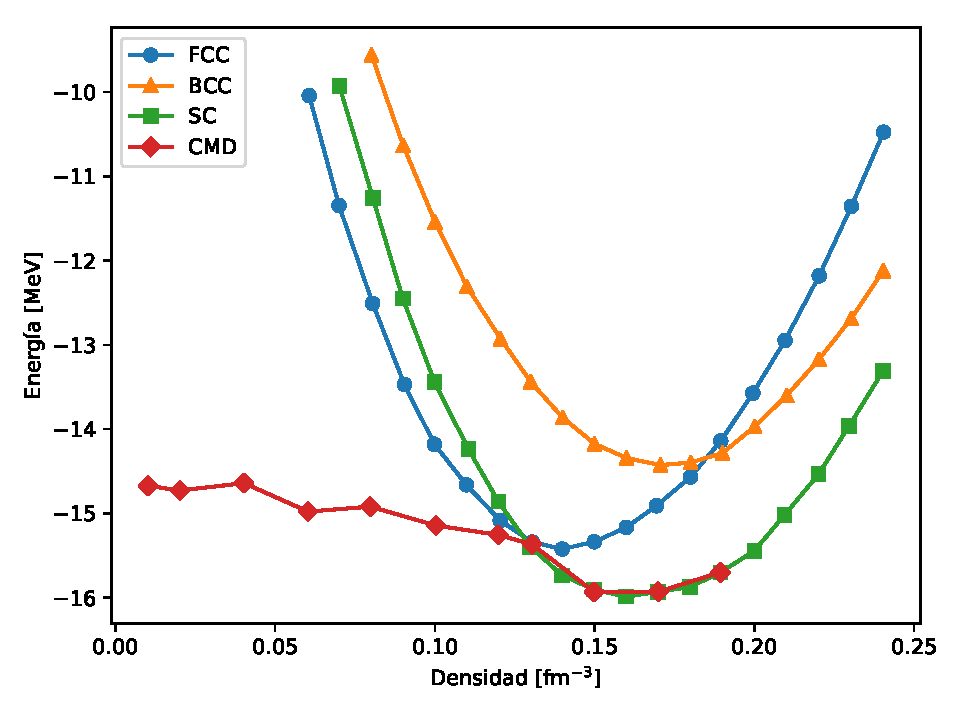
\includegraphics[width=\columnwidth]{introduccion/energy_nm}
  \caption{Energía de la materia nuclear por partícula calculada con CMD y para distintos sistemas homogéneos.}
  \label{fig:energy_nm}
\end{figure}


\begin{figure}[h]
  \centering
  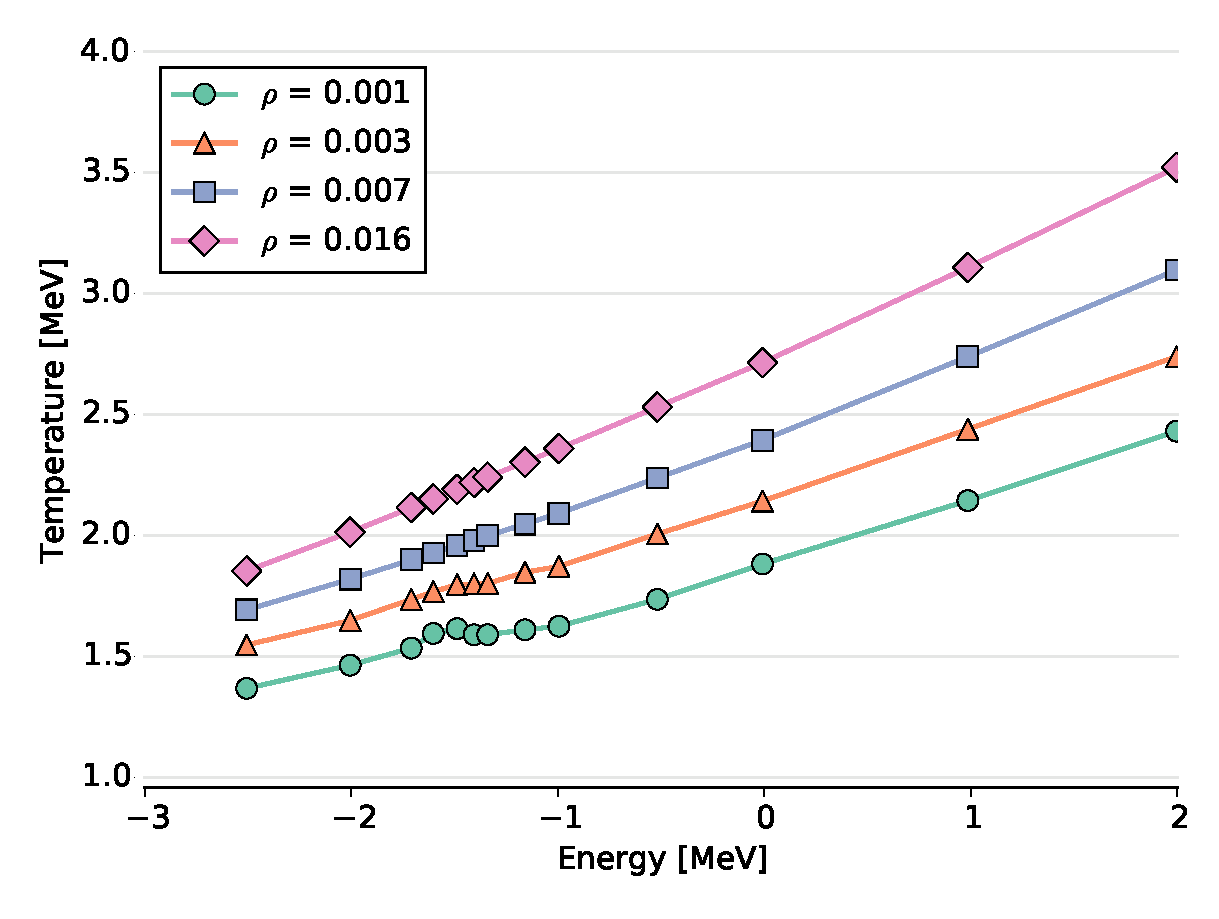
\includegraphics[width=\columnwidth]{introduccion/caloric}
  \caption{Curva calórica de un sistema equilibrado a cuatro densidades diferentes, calculado con CMD.}
  \label{fig:caloric}
\end{figure}


\subsection{Interacción de Coulomb en el Modelo}\label{sc:coulomb}

Ya que un gas de electrones neutralizante rodea a los nucleones en la corteza de las estrellas de neutrones, las fuerzas de Coulomb entre los protones son apantalladas.
El modelo que utlizamos para este efecto de apantallamiento es la aproximación de Thomas-Fermi, utilizada en varios modelos nucleares~\cite{maruyama_quantum_1998, dorso_topological_2012, horowitz_neutrino-pasta_2004}.
De acuerdo a esta aproximación, los protones interactúan a través de un potencial tipo Yukawa, con una longitud de apantallamiento $\lambda$:
\begin{equation*}
 V_{TF}(r) = q^2\frac{e^{-r/\lambda}}{r}.
\end{equation*}

Estimaciones teóricas para la longitud de apantallamiento $\lambda$ son $\lambda\sim100\,\text{fm}$~\cite{fetter_quantum_2003}, pero escogimos como valor $\lambda=20\,\text{fm}$.
Justificamos esta elección en el capítulo~\ref{ch:coulomb}, donde mostramos que este valor es suficiente para reproducir adecuadamente la longitud de las fluctuaciones de densidad para este modelo, mientras que valores mayores para la longitud de apantallamiento conllevarían a una dificultad computacional.

\section{Materia de Estrellas de Neutrones a bajas densidades y temperaturas}\label{sc:nsm_lowd}

Considerar el sistema con una interacción de Coulomb da pie a un fenómeno interesante.
A densidades menores que la de saturación, el sistema exhibe una estructura inhomogénea conocida como pasta nuclear, caracterizada por la emergencia de múltipes estructura por celda de simulación.
Esta pasta nuclear puede ser caracterizada como la originial propuesta por Williams y Koonin (ver sección~\ref{sc:intro}): \emph{gnocchi}, \emph{spaghetti}, \emph{lasagna} y túneles.
Como ejemplo, en la figura~\ref{fig:pasta} mostramos las configuraciones de algunas de estas pastas.


\begin{figure}[h]
  \begin{subfigure}[h!]{0.45\columnwidth}
    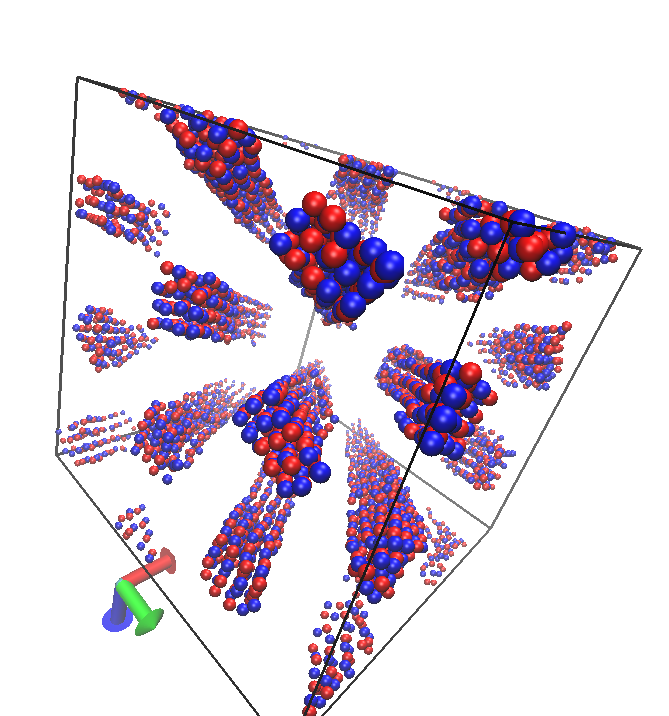
\includegraphics[width=\columnwidth]{introduccion/spaghetti}
    \caption{$\rho = 0.03\,\text{fm}^{-3}$}
    \label{sfig:spaghetti}
  \end{subfigure}
  \begin{subfigure}[h!]{0.45\columnwidth}
    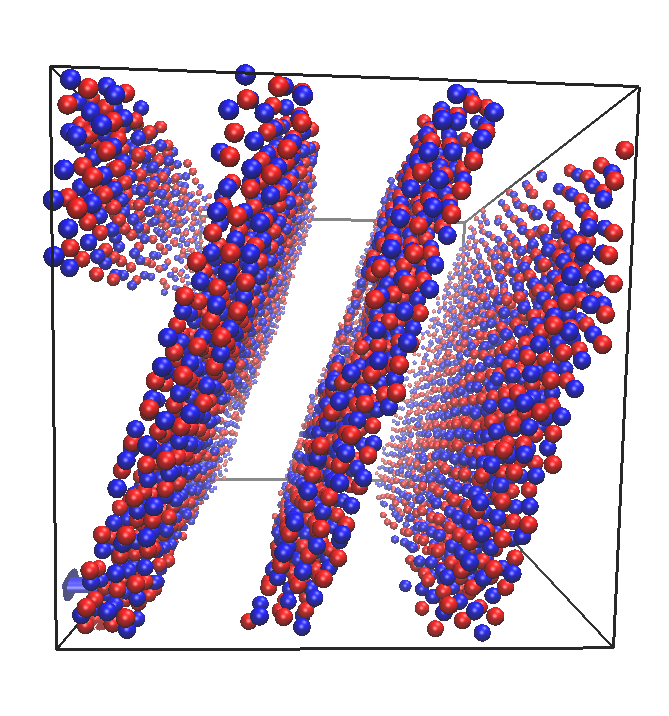
\includegraphics[width=\columnwidth]{introduccion/lasagna}
    \caption{$\rho = 0.05\,\text{fm}^{-3}$}
    \label{sfig:lasagna}
  \end{subfigure}
  \begin{subfigure}[h!]{0.45\columnwidth}
    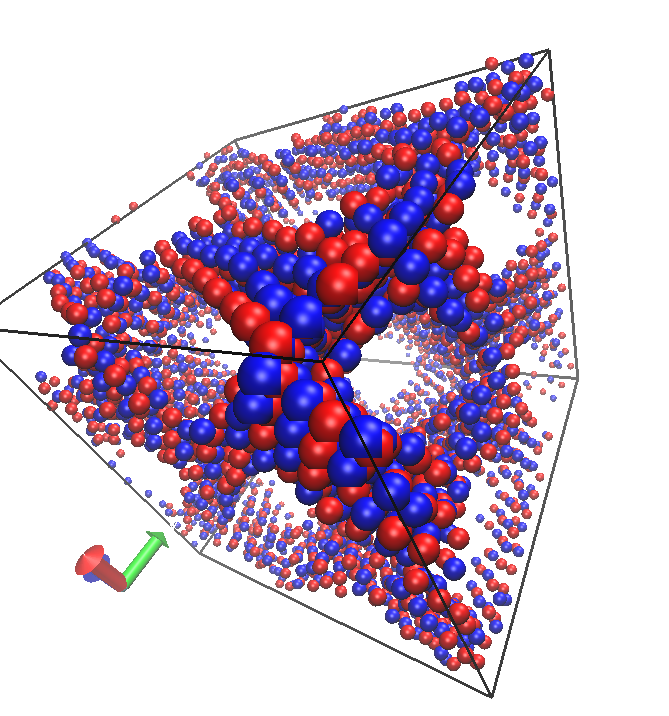
\includegraphics[width=\columnwidth]{introduccion/tunnels}
    \caption{$\rho = 0.08\,\text{fm}^{-3}$}
    \label{sfig:tunnels}
  \end{subfigure}
  \centering
  \caption{\ref{sfig:spaghetti} Spaghetti,~\ref{sfig:lasagna} lasagna y~\ref{sfig:tunnels} túneles obtenidos con CMD, para el caso simétrico en isospin $x=0.5$ y baja temperatura $T=0.5\,\text{MeV}$, extraído de Ref.~\cite{alcain_effect_2014}}
  \label{fig:pasta}
\end{figure}

% \section{Expansion}\label{sc:expansion}

% To simulate an expanding system we scale linearly with time the length
% of the box in every dimension,
% \begin{equation*}
%   L(t) = L_0 (1 + \eta\,t)
% \end{equation*}
% This, however, is not enough to expand the system collectively. We
% also need the particles inside the cell to expand like the box. In
% order to accomplish this, based on Ref.~\cite{dorso_onset_1996}, we
% add to each particle a velocity $v_{exp}$ dependent on the position in
% the box:
% \begin{equation*}
%   \mathbf{v_{exp}} = \eta\,\mathbf{r}
% \end{equation*}
% We can see from this expression that the particles in the edge of the
% box will have an expanding velocity equal to that of the box.

% Another effect to consider of this expansion is that when a particle
% crosses a boundary its velocity has to change according to the
% velocity of the expanding box. For example, if the particle crosses
% the left-hand boundary of the periodic box, the velocity of the image
% particle $v_i^\dagger$ on the right-hand must be modified $v_i^\dagger
% = v_i + L_0\,\eta$.

% \section{Cluster recognition}\label{sc:cluster}
% In typical configurations we have not only the structure known as
% nuclear pasta, but also a nucleon gas that surrounds the nuclear
% pasta. In order to properly characterize the pasta phases, we must
% know which particles belong to the pasta phases and which belong to
% this gas. To do so, we have to find the clusters that are formed along
% the simulation.

% One of the algorithms to identify cluster formation is Minimum
% Spanning Tree (MST). In MST algorithm, two particles belong to the
% same cluster $\{C^{\text{MST}}_n\}$ if the relative distance of the
% particles is less than a cutoff distance $r_{cut}$:
% \begin{equation*}
%   i \in C^{\text{MST}}_n \Leftrightarrow \exists j \in C_n \mid
%   r_{ij} < r_{cut}
% \end{equation*}

% This cluster definition works correctly for systems with no kinetic
% energy, and it is based in the attractive tail of the nuclear
% interaction. However, if the particles have a non-zero temperature, we
% can have a situation of two particles that are closer than the cutoff
% radius, but with a large relative kinetic energy.

% To deal with situations of non-zero temperatures, we need to take into
% account the relative momentum among particles. One of the most
% sophisticated methods to accomplish this is the Early Cluster
% Recognition Algorithm (ECRA)~\cite{dorso_early_1993}. In this
% algorithm, the particles are partitioned in different disjoint
% clusters $C^{\text{ECRA}}_n$, with the total energy in each cluster:
% \begin{equation*}
%   \epsilon_n = \sum_{i \in C_n} K^{CM}_i +  \sum_{i,j \in C_n} V_{ij}
% \end{equation*}
% where $K^{CM}_i$ is the kinetic energy relative to the center of mass
% of the cluster. The set of clusters $\{C_n\}$ then is the one that
% minimizes the sum of all the cluster energies $E_{\text{partition}} =
% \sum_n \epsilon_n$.

% ECRA algorithm can be easily used for small
% systems~\cite{dorso_fluctuation_1994}, but being a combinatorial
% optimization, it cannot be used in large systems. While finding ECRA
% clusters is very expensive computationally, using simply MST clusters
% can give extremely biased results towards large clusters. We have
% decided to go for a middle ground choice, the Minimum Spanning Tree
% Energy (MSTE) algorithm~\cite{dorso_topological_2012}. This algorithm
% is a modification of MST, taking into account the kinetic
% energy. According to MSTE, two particles belong to the same cluster
% $\{C^{\text{MSTE}}_n\}$ if they are energy bound:
% \begin{equation*}
%   i \in C^{\text{MSTE}}_n \Leftrightarrow \exists j \in C_n :
%   V_{ij}+ K_{ij} \le 0
% \end{equation*}
% While this algorithm doesn't yield the same theoretically sound
% results from ECRA, it still avoids the largest pitfall of naïve MST
% implementations for the temperatures used in this work.

% \subsection{Infinite Clusters}
% We developed an algorithm for the recognition of infinite clusters
% across the boundaries. We explain here in detail the implementation
% for MST clusters in 2D, being the MSTE and 3D extension
% straightforward. In figure~\ref{fig:scheme_clusters} we see a
% schematical representation of 2D clusters recognized in a periodic
% cell, labeled from 1 to 6 (note that these clusters don't connect yet
% through the periodic walls).

% \begin{figure}  \centering
%   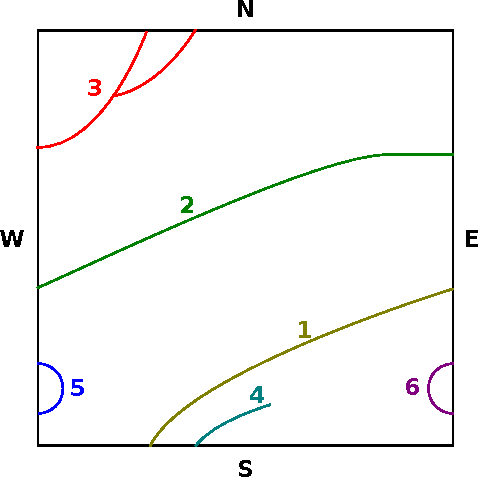
\includegraphics[width=0.75\columnwidth]{introduccion/scheme_clusters}
%   \caption{(Color online) Schematical representation of 2D clusters, recognized only
%     in the cell and not through the periodic walls, labeled as N, S,
%     W, E. The clusters inside the cell are labeled from 1 to 6,}
% \label{fig:scheme_clusters}
% \end{figure}

% In order to find the connections of these clusters through the
% boundaries, we draw a labeled graph of the clusters, where we connect
% clusters depending on whether they connect or not through a wall and
% label such connection with the wall label. For example, we begin with
% cluster 1. It connects with cluster 2 going out through the E wall,
% therefore we add a $1\rightarrow2$ connection labeled as
% E. Symmetrically, we add a $2\rightarrow1$ connection labeled as W. Now
% we go for the pair 1-3. It connects going out through the S wall, so
% we add $1\rightarrow3$ labeled as S and $3\rightarrow1$ labeled as
% N. Cluster 1 does not connect with 4, 5, or 6, therefore those are the
% only connections we have. Once we've done that, we get the graph of
% figure~\ref{fig:graph_clusters}.

% \begin{figure}  \centering
%   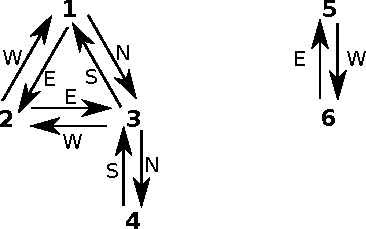
\includegraphics[width=0.45\columnwidth]{introduccion/graph_clusters}
%   \caption{Graph of the clusters with connections labeled by the wall
%     of the boundary they connect through. The graph can be divided in
%     2 subgraphs that don't connect: 1--2--3--4 and 5--6. Each of these
%     subgraphs is as cluster when periodic boundary conditions are
%     considered.}
% \label{fig:graph_clusters}
% \end{figure}

% We now wonder whether these subgraphs represent an infinite cluster or
% not not. In order to have an infinite clusters, we need to have a loop
% (the opposite is not true: having a loop is not enough to have an
% infinite cluster, as we can see in subragph 5--6), so we first
% identify loops and mark them as candidates for infinite
% clusters. Every connection adds to a loop (since the graph connections
% are back and forth), but we know from inspecting the
% figure~\ref{fig:graph_clusters} that the cluster 1--2--3 is
% infinite. Finding out what makes, in the graph, the cluster 1--2--3
% infinite is key to identify infinite clusters. And the key feature of
% cluster 1--2--3 is that its loop 1--2--3--1 can be transversed through
% the walls E--E--S, while loops like 5--6 can be transversed only
% through E--W. Now, in order for the cluster to be infinite, we need it
% to extend infinitely in (at least) one direction. So once we have the
% list of walls of the loop, we create a magnitude I associated to each
% loop that is created as follows: beginning with $I = 0$, we add a
% value $M_i$ if there is (at least one) $i$ wall. The values are: $M_E
% = 1$, $M_W = -1$, $M_N = 2$, $M_S = -2$. If $I$ is nonzero, then the
% loop is infinite. For example, for the loop E--E--S, we have E and S
% walls, so $I = M_E + M_S = 3$ and the loop is infinite. For the loop
% E--W, $I = M_E + M_W = 0$, and the loop is finite.